%!TEX root=../GaugeCNNTheory.tex


\subsection{عمل ایزومتری‌ها و تبدیل‌های گیج القا شده}
\label{sec:isometries_local}


تا کنون بحث ما منحصراً بر تقارن‌های گیج محلی در مختصات‌بندی فضاهای مماس متمرکز بوده است.
یک منیفولد ممکن است، با این حال، خود دارای تقارن‌های غیربدیهی باشد، که در مورد یک منیفولد ریمانی~$M$ \emph{گروه ایزومتری} آن $\IsomM$ را تشکیل می‌دهند.
این بخش ایزومتری‌ها و عمل آن‌ها بر منیفلدها، بردارهای مماس، چارچوب‌های مرجع و میدان‌های ویژگی را به طور خلاصه مورد بحث قرار می‌دهد، نتایجی را خلاصه می‌کند که به طور دقیق‌تری در بخش~\ref{sec:isom_background} استخراج شده‌اند.
ما بدین ترتیب معادلی بین عمل‌های \emph{فعال} ایزومتری و تفسیر \emph{منفعل} آن‌ها بر حسب تبدیل‌های گیج القا شده توسط ایزومتری را برجسته خواهیم کرد.
این معادلی بعداً امکان توصیف تناوب‌پذیری ایزومتری $\GM$-کانولوشن‌ها را فراهم خواهد کرد.


ایزومتری‌ها به عنوان تقارن‌های منیفلدهای ریمانی تعریف می‌شوند، یعنی آن نگاشت‌ها (دیفئومورفیسم‌ها)
\begin{align}
	\phi: M \to M,
\end{align}
که متریک و در نتیجه فواصل روی~$M$ را حفظ می‌کنند.
مجموعه همه ایزومتری‌های یک منیفولد ریمانی~$M$ گروه ایزومتری آن را تشکیل می‌دهد، که ما آن را با $\IsomM$ نشان می‌دهیم.
به عنوان مثال، گروه اقلیدسی~$\E{d}$ گروه ایزومتری فضاهای اقلیدسی~$\Euc_d$ است.
این گروه شامل انتقال‌ها، چرخش‌ها و بازتاب‌ها است، که همه آن‌ها متریک استاندارد~$\Euc_d$ را حفظ می‌کنند.
گروه ایزومتری 2-کره $S^2$ توسط گروه متعامد $\O3$ داده می‌شود، که شامل چرخش‌ها و بازتاب‌ها است.
شکل~\ref{fig:pushforward_vector_components} منیفولد تخم‌مرغی شکلی را نشان می‌دهد که ایزومتری‌های آن چرخش‌ها و بازتاب‌ها در $\O2$ حول محور عمودی هستند.


\begin{SCfigure}[1.8]
	\centering
	\hspace{.5ex}
	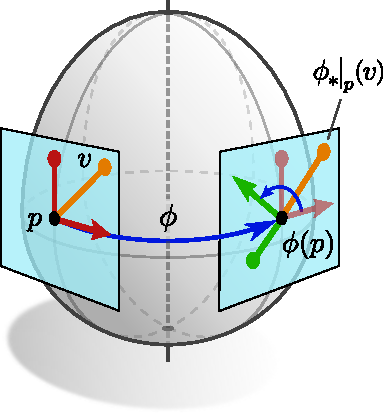
\includegraphics[width=.35\textwidth]{figures/isometry_egg_tangent_vector_gauge_trafo.pdf}
	\caption[]{\small
		بصری‌سازی پیش‌برنده آزاد از مختصات بردارهای مماس و بیان مختصاتی آن نسبت به چارچوب‌های مرجع داده شده در موقعیت منبع و هدف.
		پیش‌برنده آزاد از مختصات ${\phi_*|_p: \TpM \to \TphipM}$ بردارهای مماس $\ v \!\in\! \TpM\ $ را به $\ \phi_*|_p(v) \!\in\! \TphipM\,$ (نارنجی) منتقل می‌کند.
		فرض کنید $\psi_p^{\widetilde{A}}$ گیج در $p$ که متناظر با چارچوب مرجع قرمز است و $\psi_{\phi(p)}^A$ گیج در $\phi(p)$ که متناظر با چارچوب مرجع سبز است.
		آن‌ها بردارها را قبل و بعد از پیش‌برنده توسط ضرایب عددی $\psi_p^{\widetilde{A}}(v) = (1,1)^\top$ و $\psi_{\phi(p)}^A \big( \phi_*|_p(v) \big) = \big(0,-\sqrt{2}\big)^\top$ توضیح می‌دهند.
		این تبدیل ضرایب بردار توسط تبدیل گیج القا شده توسط ایزومتری $g_\phi^{A\widetilde{A}}(p) \in \GL{d}$ توصیف می‌شود، یعنی
		$\psi_{\phi(p)}^A \big( \phi_*|_p(v) \big) = g_\phi^{A\widetilde{A}}(p) \cdot \psi_p^{\widetilde{A}}(v)$.
		ضرایب بردارهای ویژگی به طور مشابه طبق $\rho\big( g_\phi^{A\widetilde{A}}(p) \big)$ تبدیل می‌شوند اگر $g_\phi^{A\widetilde{A}}(p) \in G$.
		\\[1ex]
	}
	\label{fig:pushforward_vector_components}
\end{SCfigure}





\subsubsection{پیش‌برنده بردارهای مماس}

هر ایزومتری $\phi \in \IsomM$ از طریق \emph{پیش‌برنده} (یا دیفرانسیل) آن
\begin{align}
	\phi_{*}|_p:\, \TpM \to \TphipM \,,
\end{align}
به طور طبیعی بر بردارهای مماس عمل می‌کند.
همانطور که در شکل~\ref{fig:intro_gauge_isom_induction} (وسط) بصری‌سازی شده است، پیش‌برنده را می‌توان به طور شهودی به عنوان حمل بردارهای مماس همراه با عمل ایزومتری بر منیفولد زیرین~$M$ در نظر گرفت.
تعریف رسمی پیش‌برنده بر روی $\TM$ در پیوست~\ref{apx:differentials_gradients_jacobians} آورده شده است، با این حال، شهود ارائه شده برای هدف ما کافی است.
از آنجا که پیش‌برنده یک نگاشت خطی آزاد از مختصات بین فضاهای مماس است، عمل آن در مختصات توسط ماتریس $d\times d$ نمایش داده می‌شود.
با فرض گیج‌های $\psi_p^{\widetilde{A}}$ و $\psi_{\phi(p)}^A$ در موقعیت منبع و هدف، به ترتیب، این ماتریس توسط
\begin{align}\label{eq:isom_induced_gauge_trafo_24}
	g_\phi^{A\widetilde{A}}(p)\ :=\ \psi_{\phi(p)}^A \circ \phi_*|_p \circ \big( \psi_p^{\widetilde{A}} \mkern1mu\big)^{-1} \ \ \in\, \GL{d} \,.
\end{align}
داده می‌شود.
این ماتریس تبدیل از ضرایب عددی یک بردار اصلی $v\in\TpM$ در گیج منبع و پیش‌برنده آن $\phi_*|_p(v) \in\TphipM$ در گیج هدف را توضیح می‌دهد، یعنی
$\psi_{\phi(p)}^A \big( \phi_*|_p (v) \big) = g_\phi^{A\widetilde{A}}(p) \cdot \psi_p^{\widetilde{A}}(v)$.
نمودار جابجایی
\begin{equation}
	\begin{tikzcd}[column sep=54pt, row sep=28pt, font=\normalsize]
		\R^d
		\arrow[dd, "g_p^{\widetilde{B}\widetilde{A}}\cdot\ "']
		\arrow[rrr, "g_\phi^{A\widetilde{A}}(p)\cdot"]
		& &[-1ex] &
		\R^d
		\arrow[dd, "\ g_{\phi(p)}^{BA}\cdot"]
		\\
		&
		\TpM
		\arrow[ul, "\psi_p^{\widetilde{A}}"]
		\arrow[dl, "\psi_p^{\widetilde{B}}"']
		\arrow[r, "\phi_*|_p"]
		&
		\TphipM
		\arrow[ur, "\psi_{\phi(p)}^A"']
		\arrow[dr, "\psi_{\phi(p)}^B"]
		\\
		\R^d
		\arrow[rrr, "g_\phi^{B\widetilde{B}}(p)\cdot"']
		& & &
		\R^d
	\end{tikzcd}
	\quad,
\end{equation}
که از نظر مفهومی شبیه آن در معادله~\eqref{cd:transporter_trivialization} است، تعریف بیان مختصاتی پیش‌برنده بردار مماس را بصری‌سازی می‌کند.
علاوه بر این دلالت دارد بر اینکه تبدیل‌های گیج بین مختصات‌بندی‌های مختلف توسط
\begin{align}
	g_\phi^{B\widetilde{B}}
	\ =\ g_{\phi(p)}^{BA} \; g_\phi^{A\widetilde{A}} \mkern1mu \big(g_p^{\widetilde{B}\widetilde{A}} \mkern1mu\big)^{-1} \,,
\end{align}
داده می‌شوند، که معادل مفهومی معادله~\eqref{eq:transporter_gauge_trafo} است.










\subsubsection{پیش‌برنده چارچوب‌های مرجع و تقارن‌های \textit{G}-ساختار}

از آنجا که چارچوب‌های مرجع فقط $d$-تاپل‌هایی از بردارهای چارچوب خطی مستقل هستند، پیش‌برنده بردارهای مماس پیش‌برنده‌ای از چارچوب‌های مرجع را با \emph{پیش‌بردن محورهای چارچوب منفرد} القا می‌کند.
به طور خاص، پیش‌برنده یک چارچوب $[e_i]_{i=1}^d$ در~$p$ به عنوان چارچوب $\big[ \phi_*|_p (e_i) \big]_{i=1}^d$ در~$\phi(p)$ تعریف می‌شود.


این پیش‌برنده چارچوب‌ها همیشه به خوبی تعریف شده است، با این حال، ممکن است با $G$-ساختار سازگار نباشد، یعنی به طور کلی تضمینی وجود ندارد که چارچوب‌ها در $\GM$ هنگام پیش‌برده شدن در $\GM$ باقی بمانند.
به عنوان مثال $\{e\}$-ساختار در شکل~\ref{fig:intro_invariant_kernel_fields_plane} (بالا چپ) را در نظر بگیرید، که توسط انتقال‌های افقی حفظ می‌شود اما توسط انتقال‌های عمودی یا هر ایزومتری دیگر از~$\R^2$ حفظ نمی‌شود.
به طور مشابه، $\Flip$-ساختار در شکل~\ref{fig:intro_invariant_kernel_fields_plane} (پایین چپ) توسط انتقال‌ها و بازتاب‌های افقی حفظ می‌شود، اما توسط چرخش‌ها نه.
بنابراین ما زیرگروه
\begin{align}\label{eq:IsomGM_def_24}
	\IsomGM\ :=\ \pig\{ \phi \in \IsomM \ \pig|\ 
	\big[\phi_*(e_i)\big]_{i=1}^d \in \GM \quad \forall\ [e_i]_{i=1}^d \in \GM \pig\} \,\ \leq\ \IsomM
\end{align}
\emph{ایزومتری‌هایی که تقارن‌های $G$-ساختار هستند} را در نظر می‌گیریم، یعنی آن‌هایی که تضمین شده‌اند هر چارچوب در~$\GM$ را به چارچوب دیگری که نیز در~$\GM$ موجود است، نگاشت کنند.%
\footnote{
	به طور رسمی‌تری بیان شود، چنین ایزومتری‌هایی \emph{اتومورفیسم‌های بندل اصلی} $G$-ساختار هستند (یا القا می‌کنند).
}
توجه داشته باشید که $\IsomGM$ به طور کلی به انتخاب خاص $G$-ساختار $\GM$ بستگی دارد، نه فقط به گروه ساختار~$G$.
برای حالت خاص که $G\geq\O{d}$، تضمین شده است که $\IsomGM=\IsomM$ مطابقت داشته باشند زیرا ایزومتری‌ها تضمین شده‌اند که چارچوب‌های متعامد را به چارچوب‌های متعامد نگاشت کنند.
ما علاقه‌مند به زیرگروه $\IsomGM$ هستیم زیرا تنها آن ایزومتری‌ها پیش‌برنده به خوبی تعریف شده‌ای از بردارهای ویژگی مستقل از مختصات $\GM$ را القا خواهند کرد، همانطور که در بخش بعدی بیشتر مورد بحث قرار گرفته است.


پیش از ادامه به عمل ایزومتری بر بردارهای ویژگی، ما آنچه را که \emph{تبدیل‌های گیج القا شده توسط ایزومتری} می‌نامیم، مورد بحث قرار می‌دهیم.
برای این منظور، فرض کنید $\big[e_i^{\widetilde{A}} \big]_{i=1}^d$ آن چارچوب در~$p$ باشد که متناظر با گیج منبع $\psi_p^{\widetilde{A}}$ است و فرض کنید $\big[e_i^A \big]_{i=1}^d$ آن چارچوب در $\phi(p)$ باشد که متناظر با گیج هدف $\psi_{\phi(p)}^A$ است، همانطور که در شکل~\ref{fig:pushforward_vector_components} به ترتیب در قرمز (چپ) و سبز (راست) نشان داده شده است.
پیش‌برنده $\big[\phi_*|_p( e_i^{\widetilde{A}}) \big]_{i=1}^d$ چارچوب منبع از $p$ به $\phi(p)$ (قرمز شفاف، راست) به طور کلی با چارچوب هدف مطابقت ندارد.
با این حال، همانطور که در بخش~\ref{sec:isom_coordinatization} اثبات شده است، دو چارچوب توسط تبدیل گیج القا شده توسط ایزومتری مرتبط هستند:
\begin{align}
	\pig[\phi_*|_p( e_i^{\widetilde{A}}) \pig] \raisebox{-2.5pt}{$\rule{0pt}{12pt}_{i=1}^d$}
	\ =\ \big[e_i^A \big]_{i=1}^d \lhd g_\phi^{A\widetilde{A}}(p) \,,
\end{align}
که در آن $g_\phi^{A\widetilde{A}}(p)$ عنصر گروهی از معادله~\eqref{eq:isom_induced_gauge_trafo_24} و $\lhd$ عمل راست از معادله~\eqref{eq:right_action_mapsto} است.
اصطلاح «تبدیل گیج القا شده توسط ایزومتری» تا آنجا معنا دارد که هندسه‌های اطراف $p$ و $\phi(p)$ غیرقابل تشخیص هستند زیرا $\phi$ یک ایزومتری، یعنی یک تقارن از~$M$ است.
با شناسایی دو نقطه با یکدیگر، بنابراین می‌توان عمل \emph{فعال} $\phi$ بر یک کمیت هندسی را به عنوان یک تبدیل گیج \emph{منفعل}، یعنی یک تغییر القا شده از چارچوب منبع به چارچوب هدف، تفسیر مجدد کرد.


قضیه~\ref{thm:isom_GM_in_coords} در بخش~\ref{sec:isom_background} اثبات می‌کند که ایزومتری‌های حفظ‌کننده $G$-ساختار در $\IsomGM$ و تبدیل‌های گیج القا شده با مقدار $G$ یکدیگر را نتیجه می‌دهند، یعنی
\begin{align}\label{eq:IsomGM_coord_in_G_24}
	\phi \in \IsomGM \quad \Longleftrightarrow \quad g_\phi^{A\widetilde{A}}(p) \in G\ \ \ \forall\ p \mkern-1mu\in\mkern-2mu M
\end{align}
برای گیج‌های دلخواه $\psi_p^{\widetilde{A}}$ و $\psi_{\phi(p)}^A$ از $G$-اطلس برقرار است.
خواننده باید این ادعاها را در مثال‌های ما در شکل~\ref{fig:intro_invariant_kernel_fields_plane} تأیید کند.






\subsubsection{پیش‌برنده بردارهای ویژگی}

اگر (و تنها اگر) یک ایزومتری تقارنی از $G$-ساختار باشد، منجر به \emph{پیش‌برنده بردارهای ویژگی} می‌شود.
به طور شهودی، این پیش‌برنده بردارهای ویژگی را از نقاط $p$ به $\phi(p)$ منتقل می‌کند.
هنگامی که نسبت به دو چارچوب مرجع در $p$ و $\phi(p)$ بیان شود، توسط تبدیل گیج القا شده
\begin{align}
	\rho\big( g_\phi^{A\widetilde{A}}(p) \big) \,.
\end{align}
داده می‌شود.
توجه داشته باشید که این تبدیل برای هر $\phi \in \IsomGM$ به خوبی تعریف شده است، زیرا تبدیل‌های گیج القا شده $g_\phi^{A\widetilde{A}}(p)$ در این حالت مقادیری در~$G$ خواهند گرفت و $\rho$ یک $G$-نمایش است.
در مقابل، اگر $\phi$ تقارنی از $G$-ساختار نباشد، تعریف پیش‌برنده بردار ویژگی متناظر \emph{غیرممکن} است.
این گزاره با این واقعیت مرتبط است که ویژگی‌های CNNهای معمولی هیچ رفتار تبدیل مشخصی تحت چرخش‌ها یا بازتاب‌ها در گروه اقلیدسی~$\E{d}$ ندارند.


پیش‌برنده بردارهای ویژگی منفرد عملی بر کل میدان ویژگی $f$ را دلالت می‌کند، که ما آن را با $\phi \rhd f$ نشان می‌دهیم.
نسبت به مختصات، این عمل به صورت
\begin{align}\label{eq:feature_field_trafo_in_coords}
	\big[\phi \rhd f\big]^A(\phi(p)) \ =\ \rho\big( g_\phi^{A\widetilde{A}}(p)\big)\, f^{\widetilde{A}}(p) \,.
\end{align}
بیان می‌شود.
ما بعداً اثبات خواهیم کرد که CNNهای مستقل از مختصات نسبت به عمل ایزومتری‌ها در $\IsomGM$ بر میدان‌های ویژگی تناوب‌پذیر هستند؛ به شکل~\ref{fig:lizard_conv_egg} مراجعه کنید.
این ویژگی بر این واقعیت تکیه دارد که عمل فعال ایزومتری بر میدان‌های ویژگی می‌تواند توسط معادله~\eqref{eq:feature_field_trafo_in_coords} به عنوان یک تبدیل گیج منفعل صرف ضرایب بردار ویژگی درک شود.